\chapter[Heuristics]{Heuristics}

% Introduction
\chapterinitial{I}{t} is often necessary to find the most desirable choice from
a large, or indeed, infinite set of options. Sometimes this can be done using
exact techniques but often this is not possible and we finding an almost perfect
choice quickly is just as good. This is where the field of heuristics comes in
to play.

\section{Problem}\label{sec:problem}

Consider a delivery company that needs to find itineraries for a driver. In
the past, the management team has noticed that drivers will often drive to
whichever next stop is closest but this often makes for longer deliveries.

The stops are represented in Figure~\ref{fig:tsp}.

\begin{figure}
    \begin{center}
        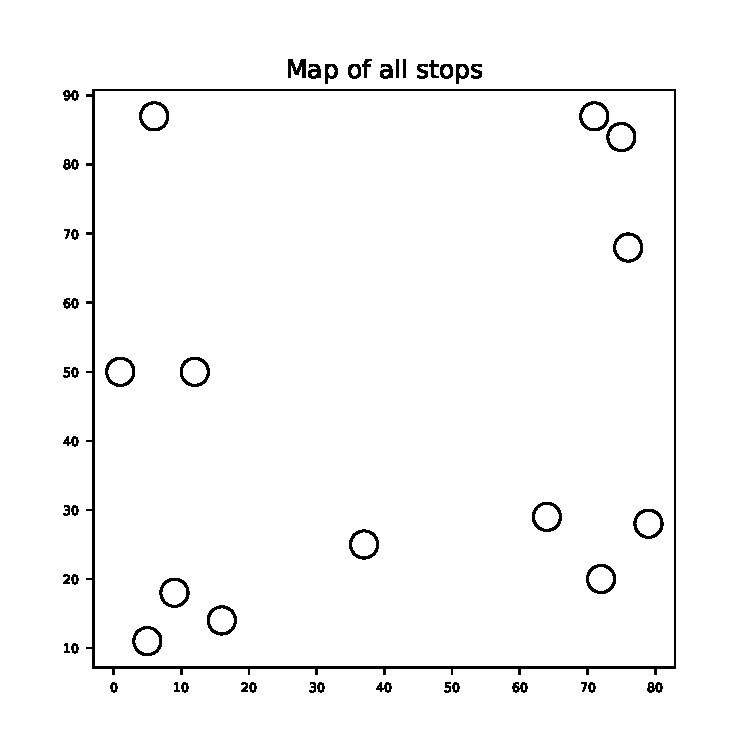
\includegraphics[width=.8\textwidth]{./assets/tsp/main.pdf}
    \end{center}
    \caption{Diagrammatic representation of the action sets and payoff matrices for
    the game.}
    \label{fig:tsp}
\end{figure}

The distance matrix is given in equation (\ref{eqn:tsp}).

\tiny{
    \chapter[Modelling with Differential Equations]{Modelling with Differential Equations}

% Introduction
\chapterinitial{S}{ystems} often change in a way that depends on their current
state. For example, the speed at which a cup of coffee cools down depends on its
current temperature. These types of systems are called dynamical systems and are
modelled mathematically using differential equations. In this chapter we will
consider a direct solution approach using symbolic mathematics.

\section{Problem}\label{sec:problem}

Consider the following situation: the entire population of a small rural town
has caught a cold. All 100 individuals will recover at an average rate of 2 per
day.  The town leadership have noticed that being ill costs approximately
\pounds10 per day, this is due to general lack of productivity, poorer mood and
other intangible aspects. They need to decide whether or not to order cold
medicine which would \textbf{double} the recover rate. The cost of of the cold
medicine is a one off cost of \pounds5 per person.
% TODO Find a more realistic example.

\section{Theory}\label{sec:theory}

In the case of this town, the overall rate at which people get better is
dependent on the number of people in how are ill. This can be represented
mathematically using a differential equation which is a way of relating the rate
of change of a system to the state of the system itself.

In general if we are interested in some variable \(x\) over time \(t\) the
differential function equation will be of the form:

\begin{equation}
    \frac{dx}{dt} = f(x)
\end{equation}

For some function \(f\).
In our case,
if we denote the number of infected individuals as \(I\) where we implicitly
mean that \(I\) is a function of time: \(I=I(t)\) and the rate at which
individuals recover by \(\alpha\) then the differential equation
that describes the above situation is:

\begin{equation}
    \frac{dI}{dt} = -\alpha I
\end{equation}

Finding a solution to this differential equation means finding an expression for
\(I\) that when differentiated gives \(- alpha I\).

In this particular case, one such function is:

\begin{equation}
    I(t) = e ^ {-\alpha t}
\end{equation}

However, \(I(0) = 1\) whereas for our problem we know that at time \(t=0\) there
are 100 infected individuals. Indeed a differential equation defines a family of
solutions and we need to know some sort of initial (also referred to as
boundary) condition to have the exact solution. Which in this case would be:

\begin{equation}
    I(t) = 100e ^ {-\alpha t}
\end{equation}

To evaluate the cost we then need to know the sum of the values of that function
over time. Integration gives us exactly this, so the cost would be:

\begin{equation}
    K \int_{0}^{\infty}I(t)dt
\end{equation}

where \(K\) is the cost per person per unit time.

In the upcoming sections we will confirm and use code to carry out the above
efficiently so as to answer the original question.

\section{Solving with Python}\label{sec:solving-with-python}

The first step we will take is to write a function to obtain the differential
equation. Note that here we will be using the Python library
\mintinline{python}{sympy} which allows us to carry out symbolic calculations.

\begin{pyin}
import sympy as sym

t = sym.Symbol("t")
alpha = sym.Symbol("alpha")
I_0 = sym.Symbol("I_0")
I = sym.Function("I")


def get_equation(alpha=alpha):
    """Return the differential equation.

    Args:
        alpha: a float (default: symbolic alpha)

    Returns:
        A symbolic equation
    """
    return sym.Eq(sym.Derivative(I(t), t), -alpha * I(t))
\end{pyin}

Using this we can get the equation that defines the population change over time:

\begin{pyin}
eq = get_equation()
print(eq)
\end{pyin}

which gives:

\begin{pyout}
Eq(Derivative(I(t), t), -alpha*I(t))
\end{pyout}

Note that if you are using Jupyter then your output will actually be a
well rendered mathematical equation:

\[
\frac{d}{d t} I{\left(t \right)} = - \alpha I{\left(t \right)}
\]

Note that we can pass a value to \(\alpha\) if we want to:

\begin{pyin}
eq = get_equation(alpha=1)
print(eq)
\end{pyin}

\begin{pyout}
Eq(Derivative(I(t), t), -I(t))
\end{pyout}

We will now write a function to obtain the solution to this differential

\begin{pyin}
def get_solution(I_0=I_0, alpha=alpha):
    """Return the solution to the differential equation.

    Args:
        I_0: a float (default: symbolic I_0)
        alpha: a float (default: symbolic alpha)

    Returns:
        A symbolic equation
    """
    eq = get_equation(alpha=alpha)
    return sym.dsolve(eq, I(t), ics={I(0): I_0})
\end{pyin}

We can verify the solution discussed previously:

\begin{pyin}
sol = get_solution()
print(sol)
\end{pyin}

which gives:

\begin{pyout}
Eq(I(t), I_0*exp(-alpha*t))
\end{pyout}

\[I(t) = I_0 e ^{-\alpha t}\]

We can use sympy itself to verify the result, by taking the derivative of the
right hand side of our solution.

\begin{pyin}
print(sym.diff(sol.rhs, t) == -alpha * sol.rhs)
\end{pyin}

which gives:

\begin{pyout}
True
\end{pyout}

All of the above has given us the general solution in terms of \(I(0)=I_0\) and
\(\alpha\) however we have written the code in such a way as we can pass the
actual parameters:

\begin{pyin}
sol = get_solution(alpha=2, I_0=100)
print(sol)
\end{pyin}

which gives:

\begin{pyout}
Eq(I(t), 100*exp(-2*t))
\end{pyout}

Now, to calculate the cost we will write a function to integrate our result:

\begin{pyin}
def get_cost(
    I_0=I_0, alpha=alpha, cost_per_person=10, cost_of_cure=0,
):
    """Return the cost.

    Args:
        I_0: a float (default: symbolic I_0)
        alpha: a float (default: symbolic alpha)
        cost_per_person: a float (default: 10)
        cost_of_cure: a float (default: 0)

    Returns:
        A symbolic expression
    """
    I_sol = get_solution(I_0=I_0, alpha=alpha)
    return (
        sym.integrate(I_sol.rhs, (t, 0, sym.oo))
        * cost_per_person
        + cost_of_cure * I_0
    )
\end{pyin}

We can now obtain the cost without purchasing the cure:

\begin{pyin}
I_0 = 100
alpha = 2
cost_without_cure = get_cost(I_0=I_0, alpha=alpha)
print(cost_without_cure)
\end{pyin}

which gives:

\begin{pyout}
500
\end{pyout}


The cost with cure can use the above with a modified \(\alpha\) and a non zero
cost of the cure itself:

\begin{pyin}
cost_of_cure = 5
cost_with_cure = get_cost(
    I_0=I_0, alpha=2 * alpha, cost_of_cure=cost_of_cure
)
print(cost_with_cure)
\end{pyin}

which gives:

\begin{pyout}
750
\end{pyout}

So given the current parameters it is not worth purchasing the cure.

\section{Solving with R}\label{sec:solving-with-R}

R has some capability for symbolic mathematics, however at the time of writing
the options available are somewhat limited and/or not reliable. As such, we will
actually solve the problem with R using a numerical integration approach. For an
outline of the theory behind this approach see Chapter % TODO Add reference to chapter

First we write a function to give us the derivative for a given value of \(I\).

\begin{Rin}
derivative <- function(t, y, parameters) {
  with(as.list(c(y, parameters)), {
    dIdt <- -alpha * I  # nolint
    list(dIdt)  # nolint
  })
}
\end{Rin}

For example, to see the value of the derivative when \(I=0\) we have:

\begin{Rin}
derivative(t = 0, y = c(I = 100), parameters = c(alpha = 2))
\end{Rin}

This gives:

\begin{Rout}
[[1]]
[1] -200

\end{Rout}

We will now make use of the \mintinline{R}{deSolve} library for solving
differential equations numerically:

\begin{Rin}
library(deSolve)  # nolint
integrate_ode <- function(times,
                          y0 = c(I = 100),
                          alpha = 2) {
  params <- c(alpha = alpha)
  ode(y = y0, times = times, func = derivative, parms = params)
}
\end{Rin}

This will return a sequence of time point and values of \(I\) at those time
points. Using this we can compute the cost. Note that this function uses
\mintinline{R}{stopifnot} to make sure our differential equation has been solved
for a long enough time period.

\begin{Rin}
get_cost <- function(
                     I_0 = 100,
                     alpha = 2,
                     cost_per_person = 10,
                     cost_of_cure = 0,
                     step_size = 0.0001,
                     max_time = 10) {
  times <- seq(0, max_time, by = step_size)
  out <- integrate_ode(times,
    y0 = c(I = I_0),
    alpha = alpha
  )
  number_of_observations <- length(out[, "I"])

  stopifnot(out[number_of_observations, "I"] < step_size)

  number_of_daily_infections <- sum(
    diff(out[, "time"]) *
      out[-number_of_observations, "I"]
  )
  number_of_daily_infections *
    cost_per_person + cost_of_cure *
      I_0
}
\end{Rin}

Using this we can compute the costs:

\begin{Rin}
alpha <- 2
cost_without_cure <- get_cost(alpha = alpha)
print(round(cost_without_cure))
\end{Rin}


which gives:

\begin{Rout}
[1] 500
\end{Rout}

The cost with cure can use the above with a modified \(\alpha\) and a non zero
cost of the cure itself:

\begin{Rin}
cost_of_cure <- 5
cost_with_cure <- get_cost(
    alpha = 2 * alpha, cost_of_cure = cost_of_cure
)
print(round(cost_with_cure))
\end{Rin}

which gives:

\begin{Rout}
[1] 750
\end{Rout}

So given the current parameters it is not worth purchasing the cure.

\section{Research}\label{sec:research}

TBA

}
\normalsize

The value \(d\) gives the travel distance between
stops \(i\) and \(j\). For example, \(d_{23}=60\) % TODO If the distance matrix changes, this value need to be updated
indicates that the distance between the 2nd and 3rd stop in the third itinerary
is given 60. % TODO If the distance matrix changes, this value need to be updated

Given these parameters, we aim to find a \emph{sufficiently good} set of
itineraries that gives a low total amount of travel.

The emphasis on needing a good solution, but not necessarily the best one,
prioritising computational efficiency is where the field of heuristics comes in
to its own.

\section{Theory}\label{sec:theory}

The heuristic approach take here will be to use a neighborhood search algorithm.
This algorithm works by considering a given potential solution, evaluating it
and then trying another potential solution \emph{close} to it. What \emph{close}
means depends on different approaches and problems: it is referred to as the
neighbourhood. As a new solution is evaluated if it is \emph{good} (this is
again a term that depends on the approach and problem) then the search
continues from the neighbourhood of this new solution.

For our problem,
the first aspect of this is to represent a given trajectory between all the
potential stops as a \emph{tour}. If we have 3 total stops and require that the
tour starts and stops at the first one then there are two possible tours:

\[
    t \in \{(1, 2, 3, 1), (1, 3, 2, 1)\}
\]

Given a distance matrix \(d\) such that \(d_{ij}\) is the distance between stop
\(i\) and \(j\) the total cost of a tour is given by:

\[
    C(t)=\sum_{i=1}^{n} d_{t_i, t_{i + 1}}
\]

Thus, with:

\[
    d = \begin{pmatrix}
        0 & 1 & 3\\
        1 & 0 & 15\\
        3 & 3 & 7
        \end{pmatrix}
\]

We have:

\begin{eqnarray*}
    c((1, 2, 3, 1)) = d_{12} + d_{23} + d_{31} = 1 + 15 + 3 = 19\\
    c((1, 3, 2, 1)) = d_{13} + d_{32} + d_{21} = 3 + 3 + 1 = 7
\end{eqnarray*}

Using this framework, the neighbourhood search can be written down as:

\begin{enumerate}
    \item Start with a given tour: \(t\).
    \item Evaluate \(C(t)\).
    \item Identify a new \(\tilde t\) from \(t\) and accept it as a replacement
        for \(t\) if \(C(\tilde t)<
        C(t)\).
    \item Repeat the 3rd step until some stopping condition is met.
\end{enumerate}

This is shown diagrammatically in Figure~\ref{fig:tsp}.

\begin{figure}[!hbtp]
    \begin{center}
        \includestandalone[width=.8\textwidth]{./assets/neighbourhood_search_flow_diagram/main}
    \end{center}
    \caption{The general neighbourhood search algorithm. \(N(t)\) refers to some
    neighbourhood of \(t\).}
    \label{fig:tsp}
\end{figure}

A number of different stopping conditions can be used including some specific
overall cost or a number of total iterations of the algorithm.

The neighbourhood of a tour \(t\) is taken as some set of tours that can be
obtained from \(t\).

To illustrate two such neighbourhoods, consider the following tour on 18 stops:
% TODO If the number of stops changes this needs to be changed.

\[
    t = (0, 2, 7, 9, 10, 14, 5, 3, 15, 11, 8, 17, 12, 4, 1, 6, 16, 13, 0)
\]

One possible neighbourhood is to choose 2 stops at random and swap. For
example, the tour \(t^{(1)}\in N(t)\) is obtained by swapping the 3rd and 8th
stops.

\[
    t^{(1)} = (0, 2, 3, 9, 10, 14, 5, 7, 15, 11, 8, 17, 12, 4, 1, 6, 16, 13, 0)
\]

Another possible neighbourhood is to choose 2 stops at random and reversing the
order
of all stops between (including) those two stops. For example, the tour
\(t^{(2)} \in N(t)\) is obtained by reversing the order of all stops between
the 9th and the 15th stop.


\[
    t = (0, 2, 7, 9, 10, 14, 5, 3, 6, 1, 4, 12, 17, 8, 11, 15, 16, 13, 0)
\]

These tours are shown in Figure~\ref{fig:tsp_example_tours}.
% TODO figure

\section{Solving with Python}\label{sec:solving-with-python}

To solve this problem using Python we will write functionality that matches the
first three steps in the Section~\ref{sec:theory}.

The first step is to write the \mintinline{python}{get_initial_candidate}
function that creates an initial tour:

\begin{pyin}
import numpy as np


def get_initial_candidate(number_of_stops, seed=None):
    """Return an initial tour.

    Args:
        number_of_stops: The number of stops
        seed: An integer seed. If an integer value is
              passed it will create a random tour.

    Returns:
        A tour starting an ending at stop with index 0.
    """
    internal_stops = list(range(1, number_of_stops))
    if seed is not None:
        np.random.seed(seed)
        np.random.shuffle(internal_stops)
    return [0] + internal_stops + [0]
\end{pyin}

Using this we can get a random tour on 18 stops:

\begin{pyin}
number_of_stops = 18
seed = 0
initial_candidate = get_initial_candidate(
    number_of_stops=number_of_stops,
    seed=seed,
)
print(initial_candidate)
\end{pyin}

\begin{pyout}
[0, 2, 7, 9, 10, 14, 5, 3, 15, 11, 8, 17, 12, 4, 1, 6, 16, 13, 0]
\end{pyout}

To be able to evaluate any given tour we see that we must also be able to
evaluate its cost. Here we define \mintinline{python}{get_cost} to do this:

\begin{pyin}
def get_cost(tour, distance_matrix):
    return sum(
        distance_matrix[current_stop, next_stop]
        for current_stop, next_stop in
        zip(tour[:-1], tour[1:])
    )
\end{pyin}

\begin{pyin}
distance_matrix = np.array(
    (
    (0, 30, 39, 28, 54, 65, 87, 81, 86, 92, 85, 34, 31, 13, 54, 53, 22, 66),
    (30, 0, 60, 14, 67, 41, 89, 79, 66, 69, 86, 61, 20, 25, 52, 34, 8, 78),
    (39, 60, 0, 65, 21, 78, 58, 59, 86, 98, 57, 16, 69, 52, 40, 61, 54, 30),
    (28, 14, 65, 0, 75, 54, 101, 91, 80, 82, 98, 62, 6, 17, 64, 48, 12, 86),
    (54, 67, 21, 75, 0, 72, 37, 39, 74, 87, 36, 37, 80, 66, 28, 56, 64, 11),
    (65, 41, 78, 54, 72, 0, 76, 62, 28, 28, 73, 86, 59, 64, 45, 17, 48, 80),
    (87, 89, 58, 101, 37, 76, 0, 15, 63, 79, 3, 74, 107, 97, 38, 64, 89, 30),
    (81, 79, 59, 91, 39, 62, 15, 0, 49, 64, 12, 74, 97, 89, 28, 51, 80, 36),
    (86, 66, 86, 80, 74, 28, 63, 49, 0, 15, 61, 98, 86, 87, 46, 33, 72, 77),
    (92, 69, 98, 82, 87, 28, 79, 64, 15, 0, 76, 109, 87, 92, 59, 40, 76, 92),
    (85, 86, 57, 98, 36, 73, 3, 12, 61, 76, 0, 73, 104, 94, 35, 61, 86, 30),
    (34, 61, 16, 62, 37, 86, 74, 74, 98, 109, 73, 0, 65, 46, 54, 70, 54, 46),
    (31, 20, 69, 6, 80, 59, 107, 97, 86, 87, 104, 65, 0, 19, 70, 54, 18, 92),
    (13, 25, 52, 17, 66, 64, 97, 89, 87, 92, 94, 46, 19, 0, 61, 54, 17, 77),
    (54, 52, 40, 64, 28, 45, 38, 28, 46, 59, 35, 54, 70, 61, 0, 30, 52, 35),
    (53, 34, 61, 48, 56, 17, 64, 51, 33, 40, 61, 70, 54, 54, 30, 0, 39, 64),
    (22, 8, 54, 12, 64, 48, 89, 80, 72, 76, 86, 54, 18, 17, 52, 39, 0, 75),
    (66, 78, 30, 86, 11, 80, 30, 36, 77, 92, 30, 46, 92, 77, 35, 64, 75, 0)
    )
)
cost = get_cost(tour=initial_candidate, distance_matrix=distance_matrix)
print(cost)
\end{pyin}

\begin{pyout}
1112
\end{pyout}

We will now define two different neighbourhood functions:

\begin{itemize}
    \item \mintinline{python}{swap_stops}: this swaps two steps in a given tour.
    \item \mintinline{python}{swap_paths}: this swaps two steps and reverts the
        stops in between them.
\end{itemize}

\begin{pyin}
def swap_stops(tour):
    number_of_stops = len(tour) - 1
    i, j = sorted(np.random.choice(range(1, number_of_stops), 2))
    new_tour = list(tour)
    new_tour[i], new_tour[j] = tour[j], tour[i]
    return new_tour

def swap_paths(tour):
    number_of_stops = len(tour) - 1
    i, j = sorted(np.random.choice(range(1, number_of_stops), 2))
    new_tour = tour[:i] + tour[i:j + 1][::-1] + tour[j + 1:]
    return new_tour
\end{pyin}

If we apply these two neighbourhood functions to our initial candidate we can
see the effects:

\begin{pyin}
print(swap_stops(initial_candidate))
\end{pyin}

which swaps the 3rd and 8th stops:

\begin{pyout}
[0, 2, 3, 9, 10, 14, 5, 7, 15, 11, 8, 17, 12, 4, 1, 6, 16, 13, 0]
\end{pyout}

\begin{pyin}
print(swap_paths(initial_candidate))
\end{pyin}

which swaps the order between the 8th and the 15th stop:

\begin{pyout}
[0, 2, 7, 9, 10, 14, 5, 3, 6, 1, 4, 12, 17, 8, 11, 15, 16, 13, 0]
\end{pyout}


Now we have all the tools in place to build a tool to carry out the
neighbourhood search \mintinline{python}{run_neighbourhood_search}.

\begin{pyin}
def run_neighbourhood_search(
    distance_matrix,
    number_of_stops,
    iterations,
    seed=None,
    get_cost=get_cost,
    get_initial_candidate=get_initial_candidate,
    get_neighbour=swap_paths,
):
    np.random.seed(seed)

    candidate = get_initial_candidate(
        number_of_stops=number_of_stops,
    )

    best_cost = get_cost(
        tour=candidate,
        distance_matrix=distance_matrix,
    )

    for _ in range(iterations):
        new_candidate = get_neighbour(candidate)
        if (cost:=get_cost(
                    tour=new_candidate,
                    distance_matrix=distance_matrix,
                  )
            ) <= best_cost:
            best_cost = cost
            candidate = new_candidate

    return candidate
\end{pyin}

Using this we can see the effect of running 1000 iterations using different
neighbourhood functions:


\begin{pyin}
number_of_iterations = 1000

solution_with_swap_stops = run_neighbourhood_search(
    distance_matrix=distance_matrix,
    number_of_stops=number_of_stops,
    iterations=number_of_iterations,
    seed=seed,
    get_neighbour=swap_stops,
)
print(solution_with_swap_stops)
\end{pyin}

giving:

\begin{pyout}
[0, 2, 4, 17, 6, 10, 7, 14, 8, 9, 5, 15, 1, 16, 3, 12, 13, 11, 0]
\end{pyout}

\begin{pyin}
solution_with_swap_paths = run_neighbourhood_search(
    distance_matrix=distance_matrix,
    number_of_stops=number_of_stops,
    iterations=number_of_iterations,
    seed=seed,
    get_neighbour=swap_paths,
)
print(solution_with_swap_paths)
\end{pyin}

giving:

\begin{pyout}
[0, 13, 12, 3, 16, 1, 5, 9, 8, 15, 14, 7, 10, 6, 17, 4, 2, 11, 0]
\end{pyout}

Importantly the costs differ substantially:

\begin{pyin}
print(get_cost(tour=solution_with_swap_stops, distance_matrix=distance_matrix))
\end{pyin}

which gives:

\begin{pyout}
409
\end{pyout}

Whereas using the entire swapping of paths % TODO Refer to name of algorithm.

\begin{pyin}
print(get_cost(tour=solution_with_swap_paths, distance_matrix=distance_matrix))
\end{pyin}

which gives:

\begin{pyout}
360
\end{pyout}

% TODO initial, swap stops and swap paths

\section{Solving with R}\label{sec:solving-with-R}

\section{Research}\label{sec:research}

TBA
